\subsection{Android application}
\chapterauthor{Theolin, Henrik (Axelsson, Oskar)}
The main reason for this project is to give a sailor qualitative feedback and help in clearing the mind of the techniques required to achieve a smooth sail experience so that the sailor can focus on the joy of sailing.
A crucial part is to display the data in a manner that is easy to interpret and provide the help that the skipper needs.

To further increase the flexibility of the design, several different user layouts are implemented, that the user can switch between while running the application. This was determined to be a good way of increasing the chances that the user would find a preferable layout.

It was also determined that not only visual representation was enough, since the sailor needs to be in constant motion to counteract the forces applied on the ship by the wind and currents. This will make watching a screen to retrieve information somewhat difficult.
Other ways of representing data were implemented using text-to-speech where the sailor will get important information by sound as well as text
 Vibration is also implemented with different vibration sequences depending on different states of the ship.


\subsubsection{Software design}
A \gls{uml}\cite{uml} model of the system, see \autoref{android-uml}, was developed for an overview of the system implementation. The android system uses activities\cite{activity} to display content to the device screen. These activities have a life-cycle (\autoref{android-activity}) that determine how data is accessed and displayed. What should be understood is that the application starts in a main activity, and switching to another activity is done by sending an intent that spawns as a child activity.
While the application is in the child activity the main activity is paused but the state is stored and when switching back from the child all data from the previous state is being accessed.
When the user returns from the child activity,  that activity is destroyed and all data is erased.
Sending data between activities is done using intents, to send an intent to a child activity is done by adding a bundle with a data object along with the intent to spawn the child activity.
Sending data back to the child activity is done by calling the method ``\emph{startActivityForResult}'', this allows the child to send a data packet as a result back to the parent. 
\begin{figure}[H]%Can this be put in the Appendix? It is very large and detailed.
\centering
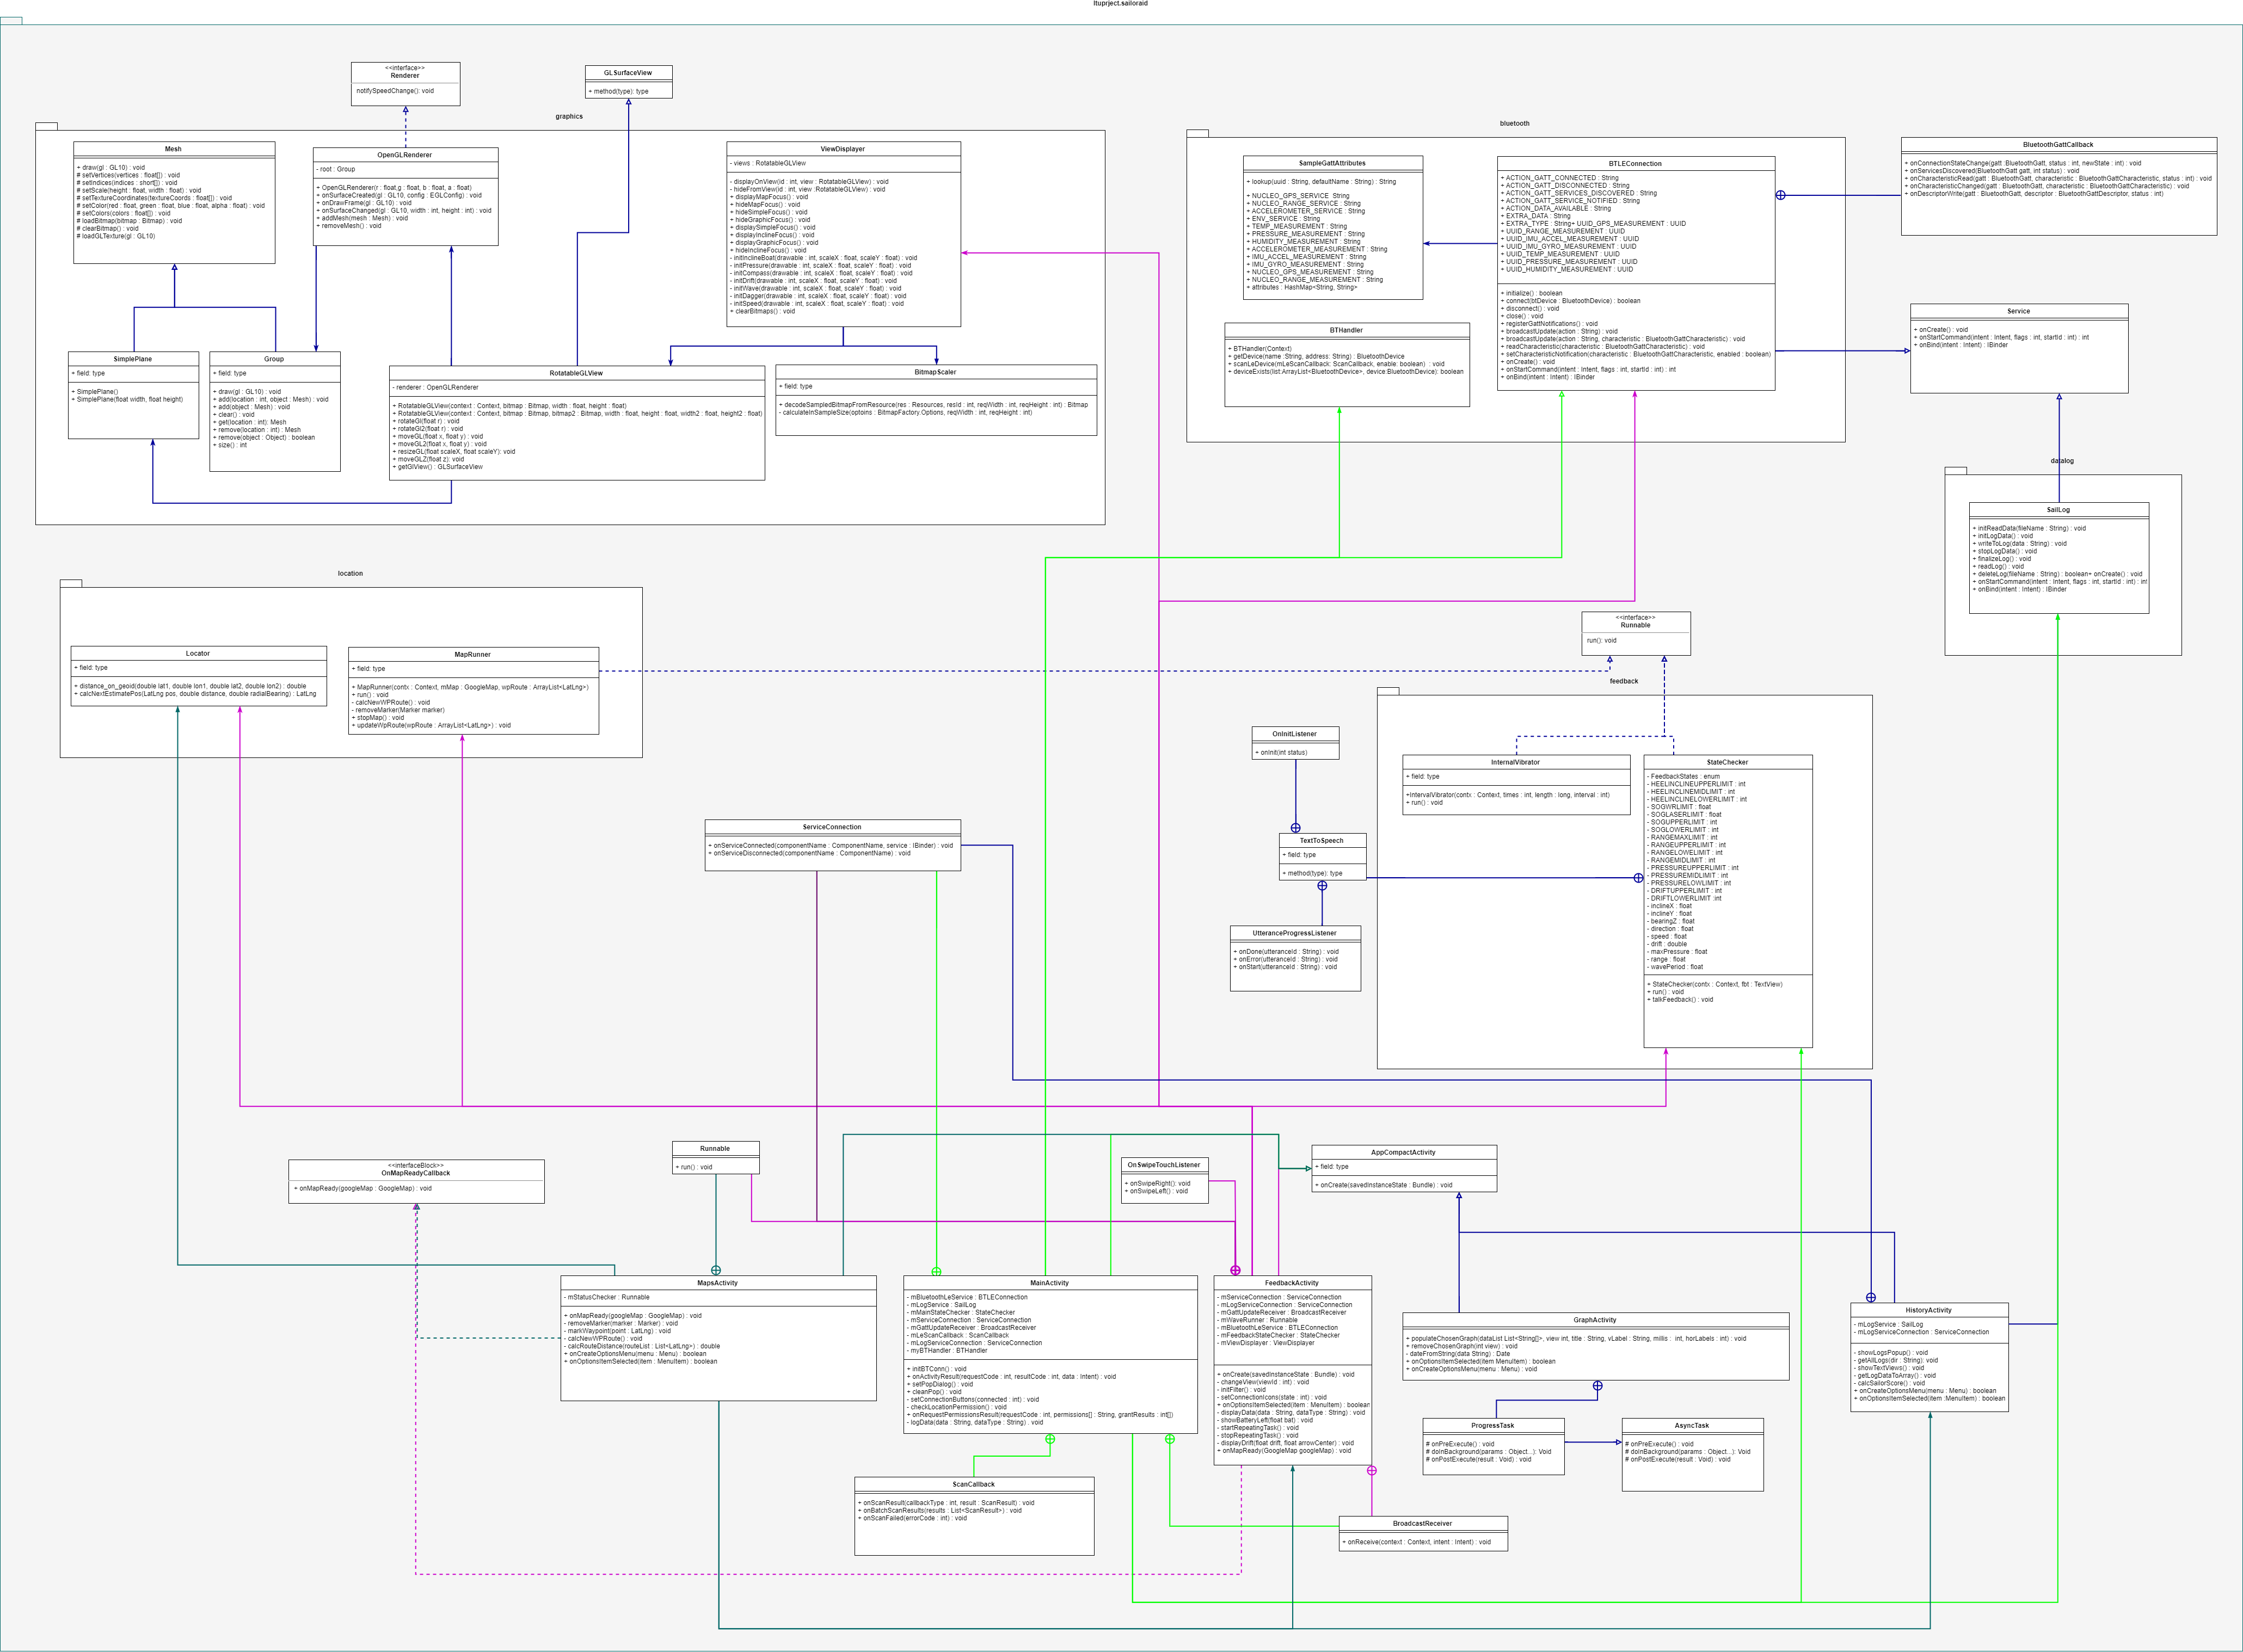
\includegraphics[width=\textwidth]{Figures/uml.png}
\caption{\gls{uml} model.}
\label{android-uml}
\end{figure}
\begin{figure}[H]
\centering
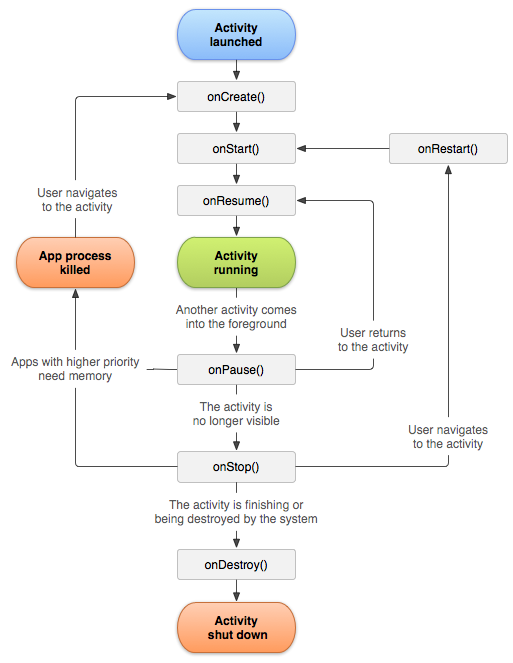
\includegraphics[width=0.8\textwidth]{Figures/activity_lifecycle.png}
\caption{Activity lifecycle.}
\label{android-activity}
\end{figure}

The Bluetooth connection and data logging class is implemented as a services\cite{android-service}. A service can be started by an activity and continue running until it is explicitly called to stop. This allows several activities to share resources and perform long-running operations in the background. The lifecycle of a service is seen in \autoref{android-service}.
\begin{figure}[H]
\centering
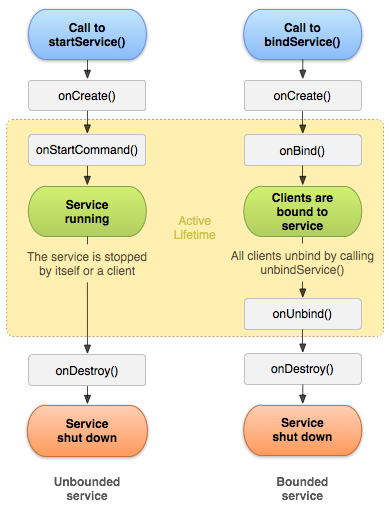
\includegraphics[width=0.8\textwidth]{Figures/service_lifecycle.png}
\caption{Activity lifecycle.}
\label{android-service}
\end{figure}

\subsubsection{Feedback}
For the feedback states in the application, there are some approximations, and simplifications made for easier implementation. As explained in \autoref{sec:physics}, the chapter about Physics of sailing, there are certain parameters that can be evaluated in different states of the dinghy. An extensive approximation is that there is no water movement in the implementations. The states implemented are
\begin{labeling}{alligator}
\item [Clear] - The dinghy holds good velocity and not heeling or drifting and with a good amount of pressure on the dagger-board
\item [Drift] - The dinghy is drifting perpendicular to the bearing while the dagger-board is in an upper position
\item [Heel] - The dinghy has high heel angle
\item [Reefing] - The dinghy has high heel angle and the pressure on the dagger-board is high
\item [Wrspeed] - The dinghys speed is above $65.45~\textrm{kn}$
\item [Lrspeed] - The dinghys speed is above $16.8~\textrm{kn}$
\item [Hike] - The dinghy has more then moderate heel angle and the pressure on the dagger-board is between medium and high
\item [Keelhaul] - The dinghy has an above moderate heel angle and the dagger-board is not in the lowest position
\item [Runninghigh] - The dinghy is sailing directly windwards with dagger-board high and low heel angle.
\item [Runninglow] - The dinghy is sailing directly windwards with dagger-board high and mid heel angle.
\item [Landcrab] - The dinghys speed is low.
\end{labeling}
Given these states, appropriate feedback can then be provided to the user. For handling states, a class called \emph{StateChecker} was implemented. This stores sensor values and check against limits defined at an interval that is also defined in the class. Depending on these states this class also determines what feedback that should be given.

\subsubsection{Visual Feedback}
It was determined that the visual feedback provided to the user was to include very little text information and would consist mainly of figures that changed position based on sensor data to give a good representation of what was going on with the dinghy. Because of different personal preferences, the ability to switch between different layouts is implemented. This is done by a simple swipe on the screen to toggle the view to the next layout. All layouts consists of a subset of views from the complete set including
\begin{labeling}{alligator}
\item [\ref{feedback-incline} \textbf{Incline}]  displays a ships relative incline against and artificial horizon.
\item [\ref{feedback-pressure} \textbf{Pressure}] moves a pin along a colored bar to represent high of low pressure applied on the dagger-board.
\item [\ref{feedback-compass} \textbf{Bearing}] rotates a compass to show the ship relative bearing against true north.
\item [\ref{feedback-map} \textbf{Map}] displays current location of the ship.
\item [\ref{feedback-height} \textbf{Speed}] displays a speedometer from a classical Swedish vehicle\cite{volvo} with a movable bar representing speed over ground.
\item [\ref{feedback-drift} \textbf{Drift}] is represented with a colored bar containing two arrows that moves to the relative drift direction to show the sailor if the ship was holding its set navigational reference.
\item [\ref{feedback-text} \textbf{Feedback}] a text that changes values based on the current state of the boat.
\item [\ref{feedback-sog} \textbf{Height}] of the dagger-board is represented with a visual dagger-board moving up and down along a graphical ruler.
\item [\ref{feedback-wave} \textbf{Wave frequency}] displays a wave moving towards a ship at a speed representing different period of the waves.
\end{labeling}

\begin{figure}[H] 
 	\centering
	\begin{minipage}[c]{0.6\textwidth}
	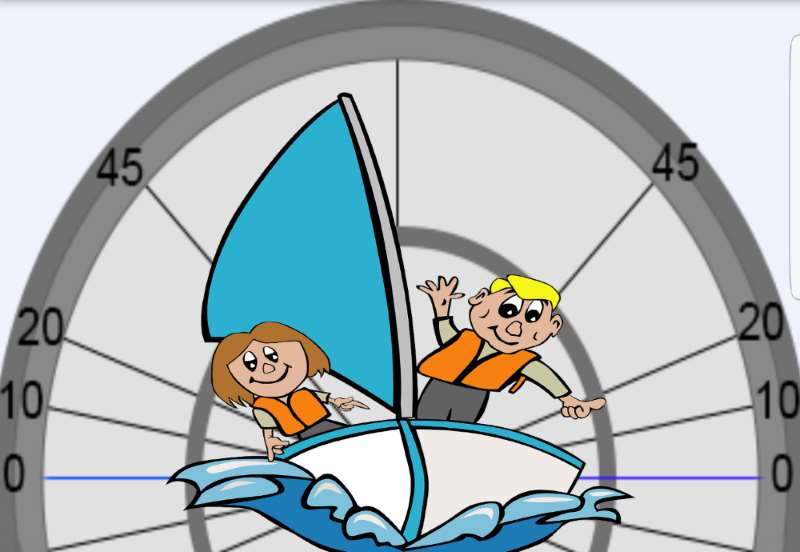
\includegraphics[width=\textwidth]{Figures/incline.jpg}
	\caption{Incline feedback view}
	\label{feedback-incline}
	\end{minipage}
	~
	\begin{minipage}[c]{.3\textwidth}
	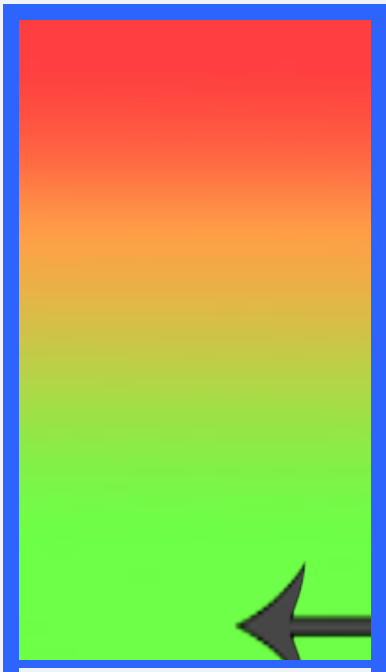
\includegraphics[width=\textwidth]{Figures/pressure.png}
	\caption{Pressure feedback view.}
	\label{feedback-pressure}
	\end{minipage}
\end{figure}
%
\begin{figure}[H]
	\centering
	\begin{minipage}[c]{0.55\textwidth}
	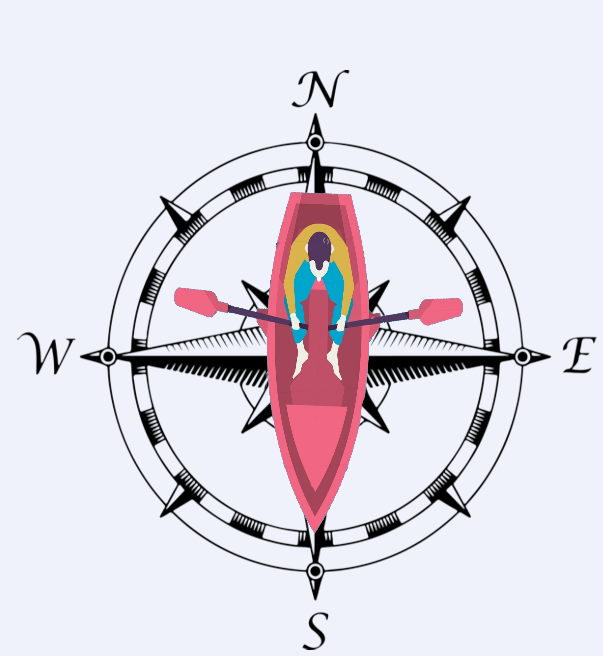
\includegraphics[width=\textwidth]{Figures/compass.png}
	\caption{Bearing feedback view.}
	\label{feedback-compass}
	\end{minipage}
	~
	\begin{minipage}[c]{0.35\textwidth}
	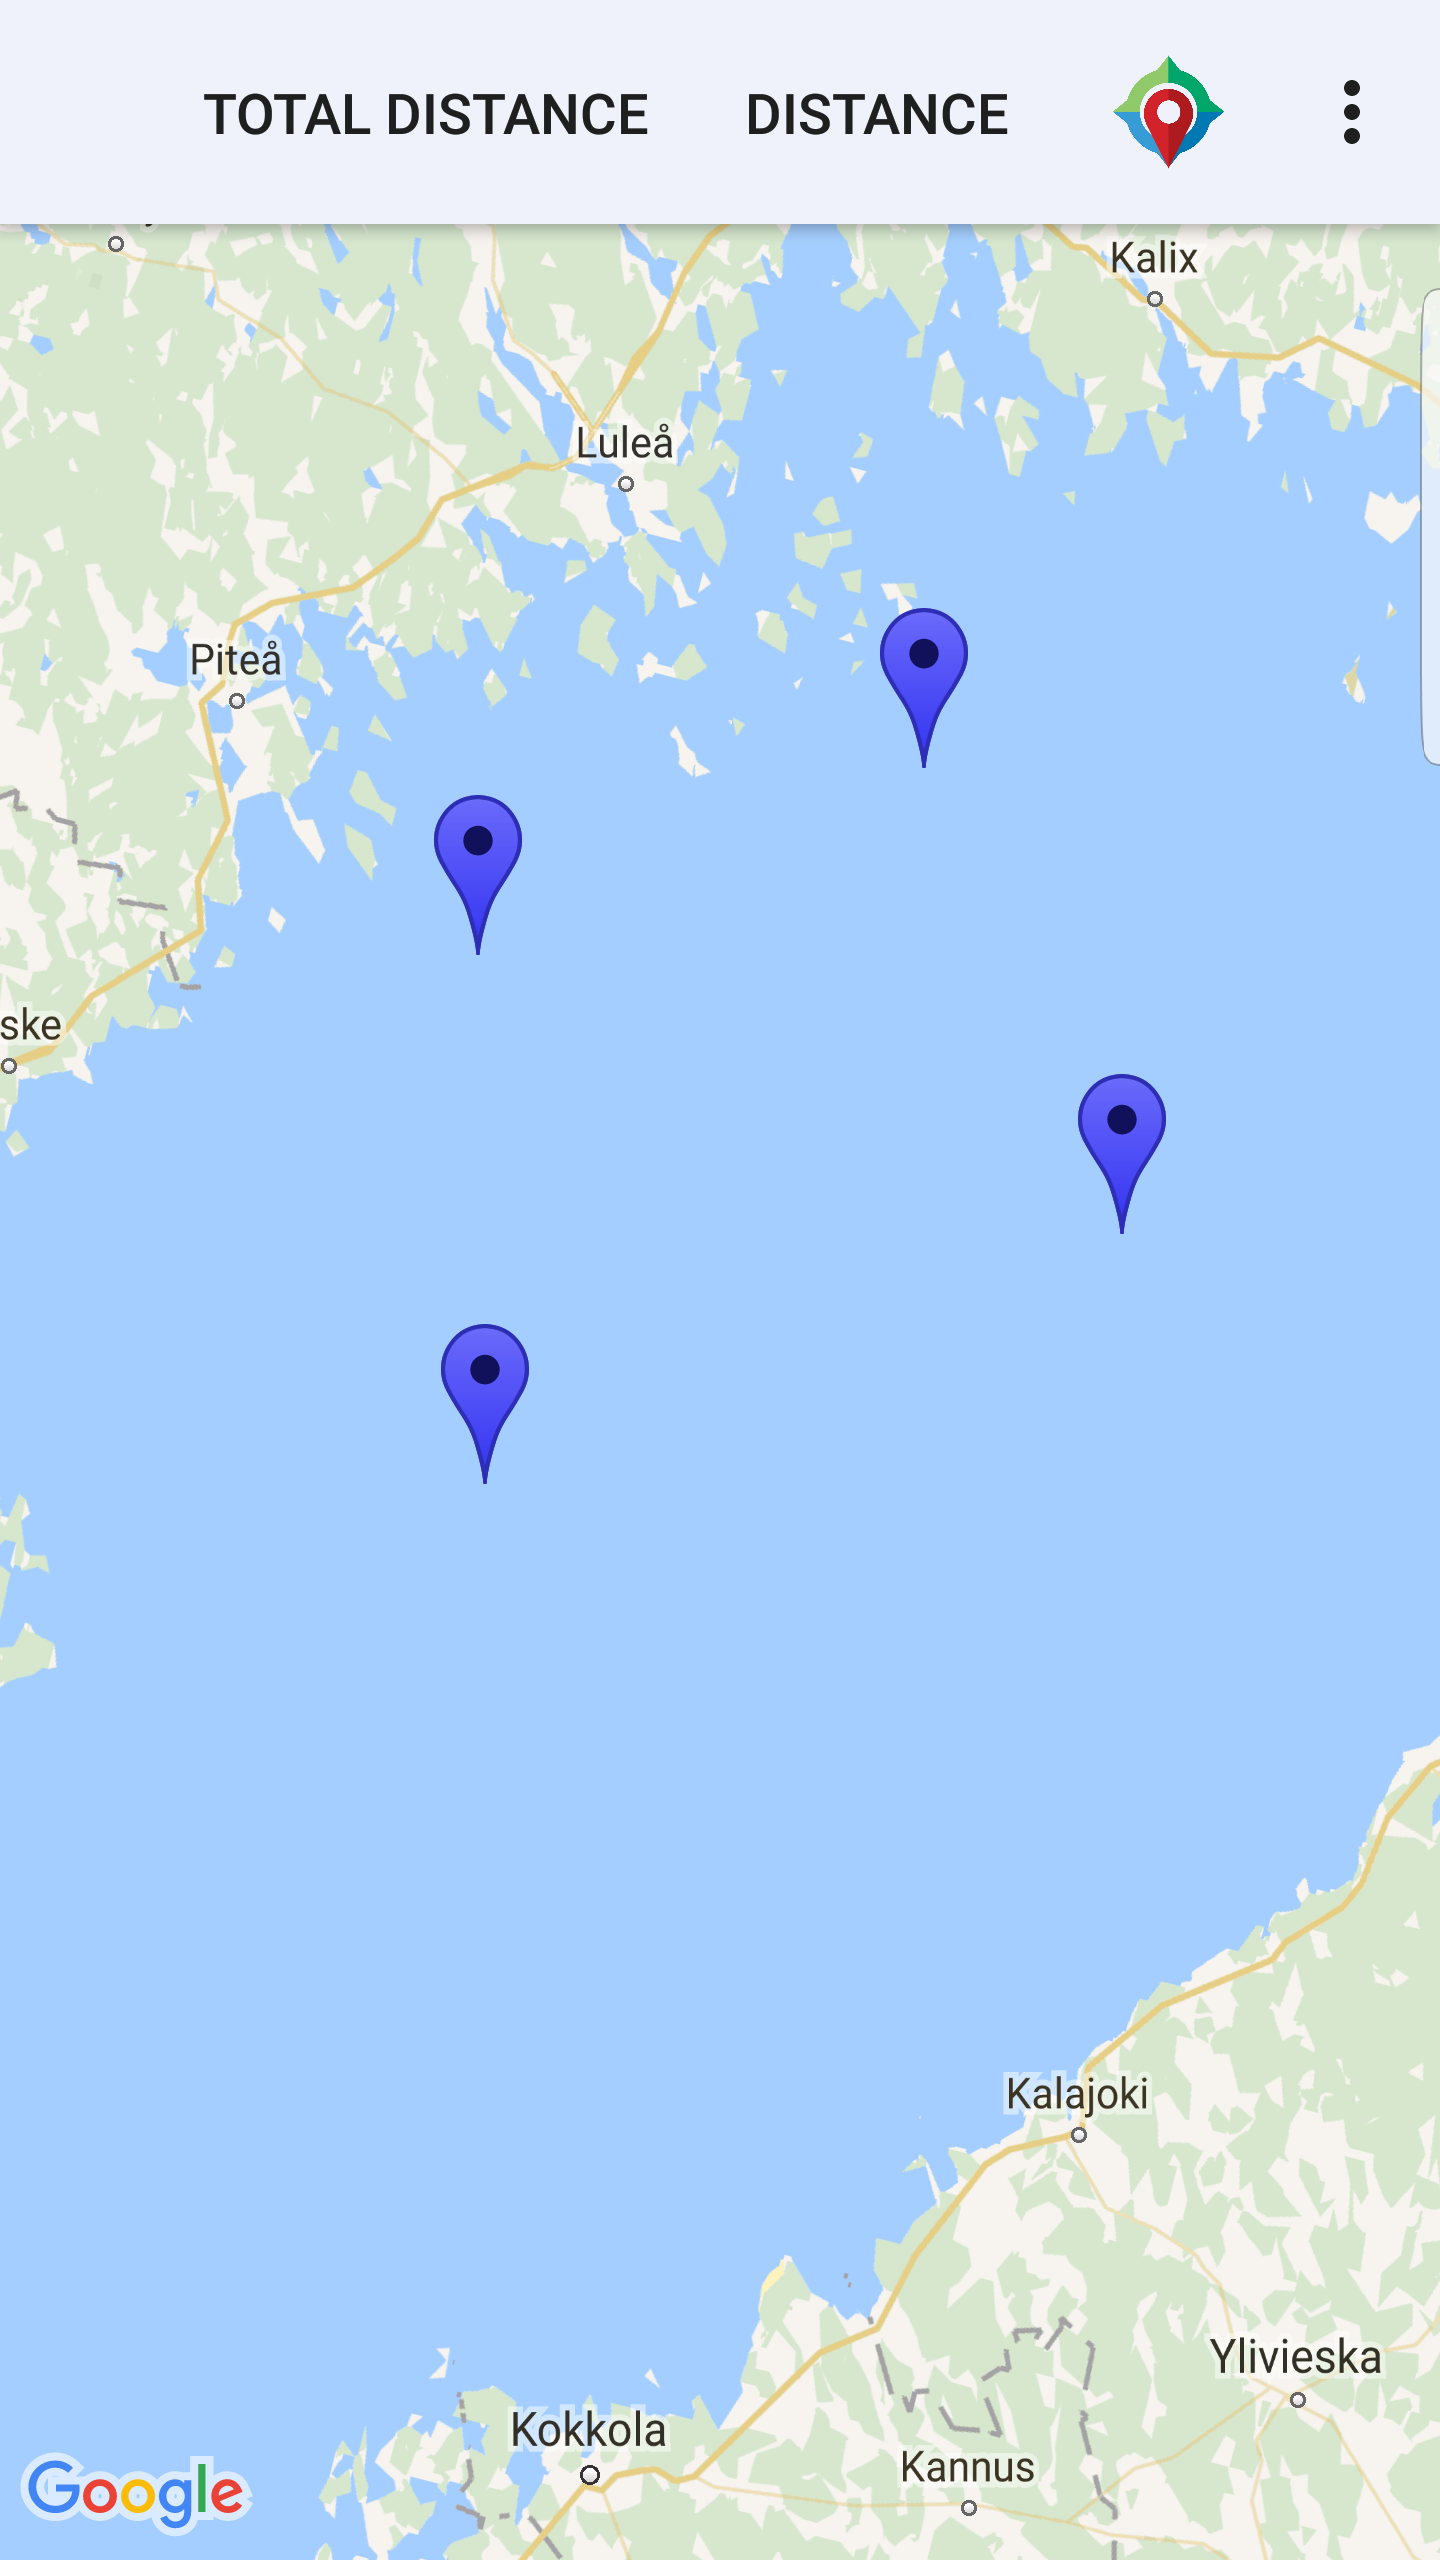
\includegraphics[width=\textwidth]{Figures/map.png}
	\caption{Map feedback view.}
	\label{feedback-map}
	\end{minipage}
\end{figure}
\begin{figure}[H]
	\centering
	\begin{minipage}[c]{0.35\textwidth}
	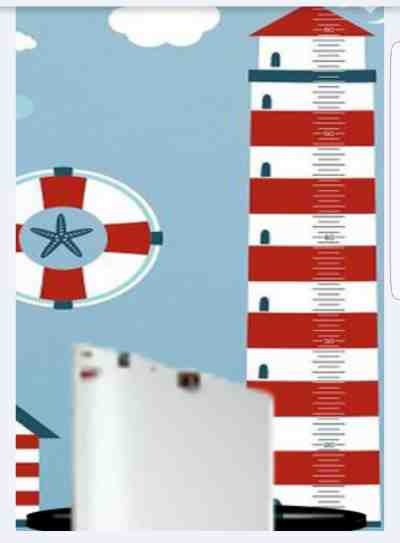
\includegraphics[width=\textwidth]{Figures/height.jpg}
	\caption{Dagger-board height view.}
	\label{feedback-height}
	\end{minipage}
	~
	\begin{minipage}[c]{0.55\textwidth}
	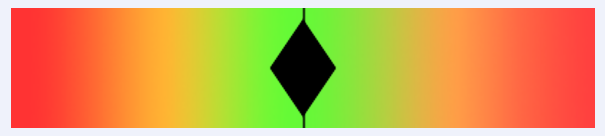
\includegraphics[width=\textwidth]{Figures/drift.png}
	\caption{Drift feedback view.}
	\label{feedback-drift}
	
	
\includegraphics[width=\textwidth]{Figures/text.png}
	\caption{Text feedback view.}
	\label{feedback-text}
	\end{minipage}
\end{figure}
\begin{figure}[H]
	\centering
	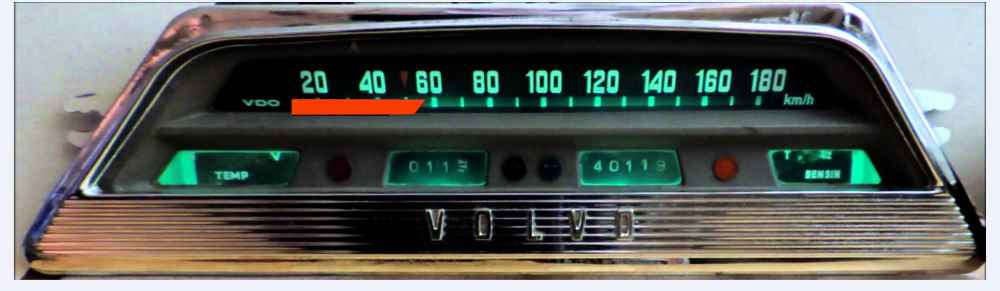
\includegraphics[width=0.8\textwidth]{Figures/sog.jpg}
	\caption{Speed over ground view.}
	\label{feedback-sog}
\end{figure}
\begin{figure}[H]
	\centering
	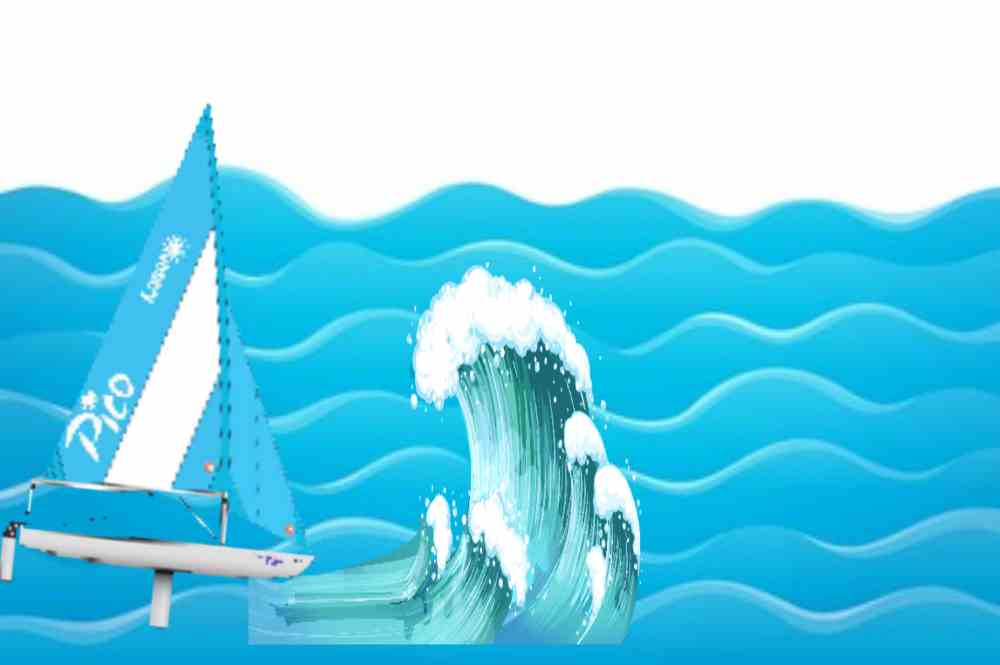
\includegraphics[width=0.8\textwidth]{Figures/wave.jpg}
	\caption{Wave period feedback view.}
	\label{feedback-wave}
\end{figure}
The figures were chosen at a development stage and improvements can easily be made by adding different \gls{png}\cite{png} files in android studio. They are implemented as \emph{GLSurfaceView}\cite{gl} so that updating the figures is be done by calling a \emph{requestRender} function, this improves the performance of the application when only updates to the figures are done when new sensor readings are received. To make the figure fit the application the \emph{GLSurfaceView} is extended into a \emph{RotatableGLView} that has the wanted features for rotation and positioning. Using these figures four different layouts are developed to give multiple choices for the user and is seen in figure \ref{feedback-layouts}. Switching between these layouts a \emph{swipeTouchListener} is implemented which allows the user to swipe across the screen to change the layout. Changing view the figures needs to be redrawn onto a new view matching the current layout, this is handled in the \emph{ViewDisplayer} class that contained all \emph{RotatableGLViews}.

\begin{figure}[H]
\centering
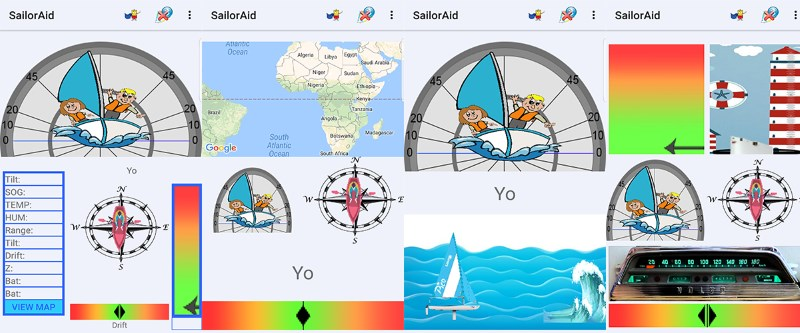
\includegraphics[width=0.9\textwidth]{Figures/layouts.jpg}
\caption{Different layouts}
\label{feedback-layouts}
\end{figure}

\subsubsection{Audio feedback}
Based on values from the sensors, different states are implemented and for each state, a text is read out to the user. The feedback is implemented such that the audio feedback would continue even if the device is put into sleep mode. Handling the text to speech feature a \emph{Text-to-Speech}\cite{texttospeech} class is implemented as an inner class in \emph{StateChecker}. To prevent the speech to be interrupted preemptively an \emph{UtteranceProgressListener}\cite{utter} is used. 

\subsubsection{Haptic feedback}
Based on the same states as the audio feedback vibration is also implemented. The frequency and length of the vibrations are implemented in such a way each state has a unique signature that can be recognized by the sailor after some practice with the system. Handling the interval an \emph{IntervalVibrator} is implemented and run by the \emph{StateChecker}.

\subsubsection{Log}
The ability to analyze the sailing trip was determined to be an important feature for the user, so a logging function is implemented so data can be stored in the device internal storage. This is handled by the \emph{SailLog} class and these files can be read or deleted at a later stage, by the user. Storing a log is implemented such that the sailor would need to start a logging session after Bluetooth connection has been established to the ship. After the log is started it creates a file on the device internal storage and writes sensor data to the file at the same frequency as the data is transmitted by the system. While logging is active the device would continue to store information even if the device is put in sleep mode so that the sailor could choose to only log data and not view the information displayed on the screen. After the sailing trip is finished the sailor can read the saved log file and receive a summary of the trip (\autoref{log-summary}). More information from the log can be analyzed by reading graphs (\autoref{log-graph}) where the sensor data is shown with respect to time. These graphs are implemented such that the user is able to choose what graphs to be displayed on the device for improved comparability.
\begin{figure}[H]
	\centering
	\begin{minipage}[t]{0.3\textwidth}
	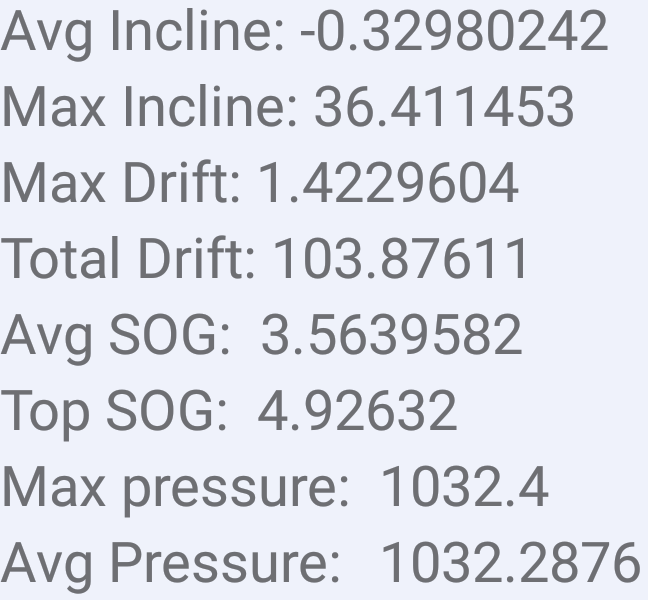
\includegraphics[width=\textwidth]{Figures/log_data.png}
	\caption{Log data summary example.}
	\label{log-summary}
	\end{minipage}
	~
	\begin{minipage}[t]{0.6\textwidth}
	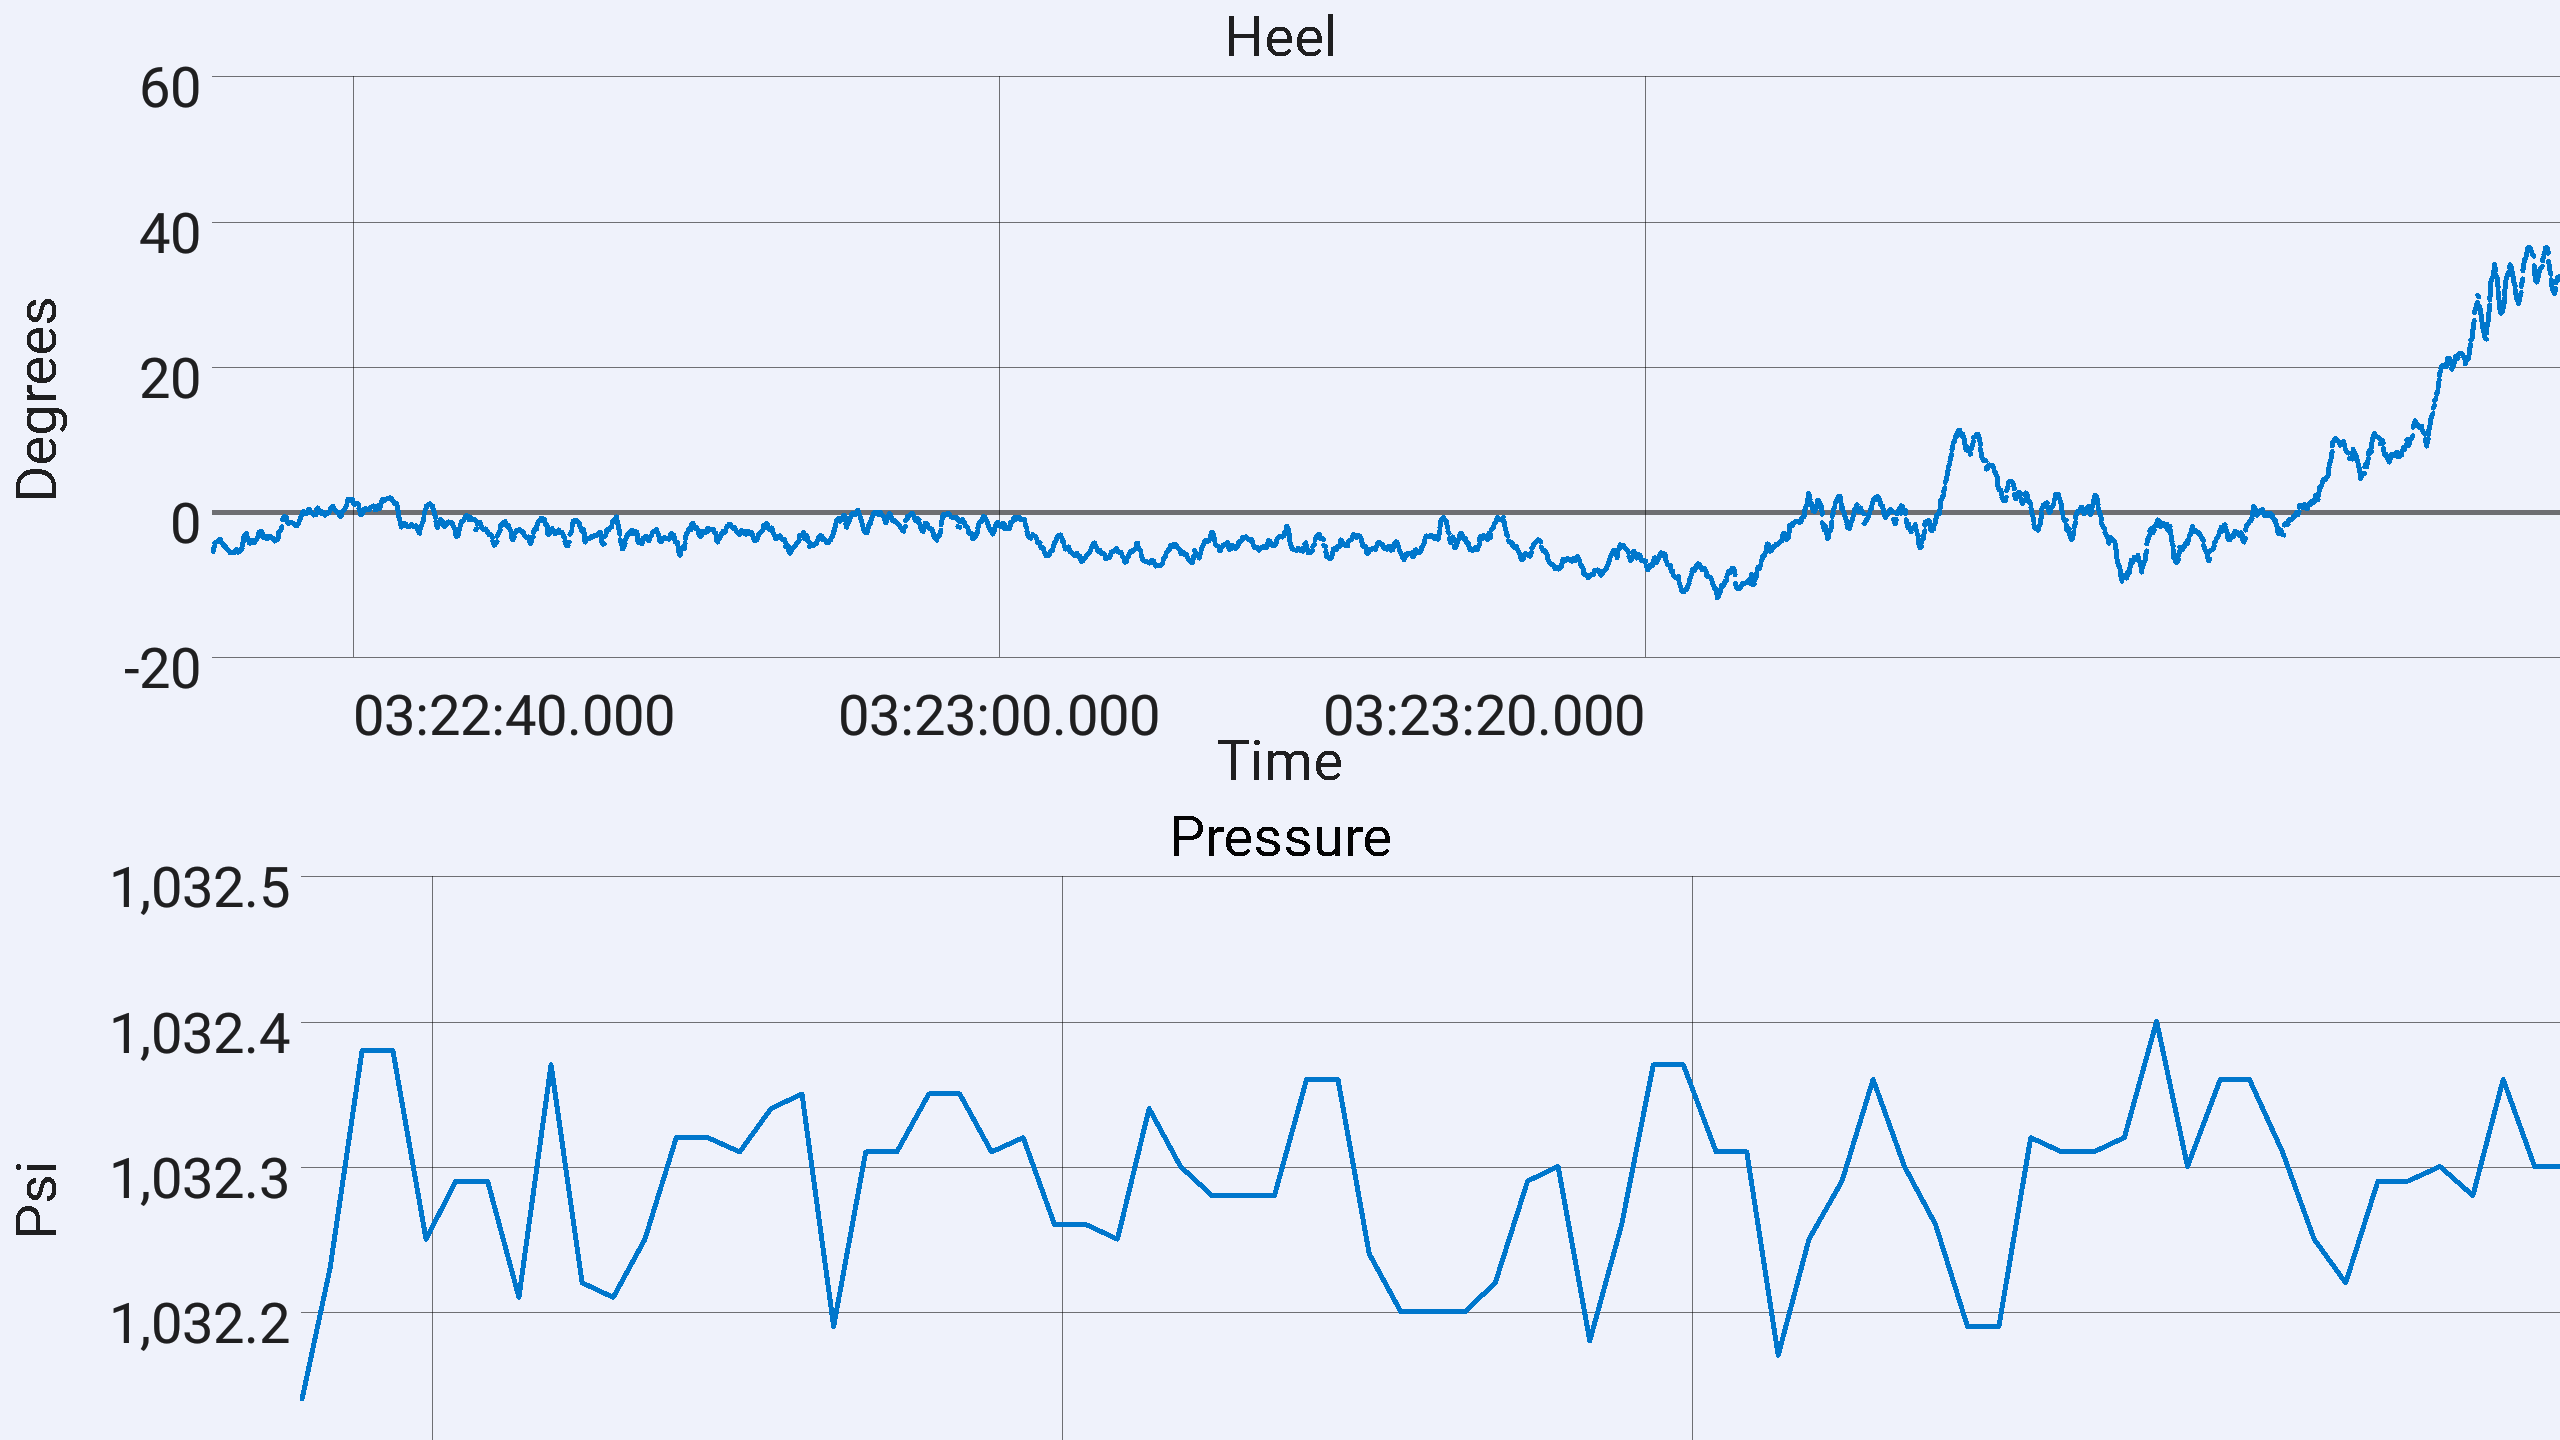
\includegraphics[width=\textwidth]{Figures/log_graph.png}
	\caption{Log graphs examples.}
	\label{log-graph}
	\end{minipage}
\end{figure}

\subsubsection{Bluethooth connection}
A list of all devices in the nearby area is displayed when the user decides to connect to the system, this adds flexibility to the user and allows for connection between multiple systems with different \gls{mac}. Scanning for nearby devices is done in the \emph{MainAcivity} and handled by the \emph{BTHandler} class. The application uses Bluetooth low energy technology to match the system implementation. This allows the device to receive notifications when the data is altered on the system and updates occurs in different frequencies for different types of data. To ensure a stable connection between the system and the device the connection class is implemented as an android service\cite{android-service}. This allows the device to keep the connection alive between different views and even when the device is put into sleep mode. All functionality regarding connecting and receiving data is implemented in the \emph{BTLEConnection} class and known characteristics and the determined unique GATT service identifiers are stored in the \emph{SampleGattAttributes} class.

\subsubsection{Map}
For the sailor to get more information about location two maps are implemented, one that is embedded into a layout in the \emph{FeedbackActivity} and the functionality of this is handled in the \emph{MapRunner} class, the other map is implemented in \emph{MapsActivity}. This could be improved by using the same class for both maps to achieve better readability and modifiability of the code. Both these implementations utilized the Google maps \gls{api}\cite{gmaps}, which can be used freely and the map service is highly accurate and suits our system well. Interaction with the maps can also be made quite easy which helped to make development faster. The sailor has the ability to see a path over the trip and the total distance traveled. Waypoints can be placed if the sailor wants to plan a certain trip in advance. The distance of the trip and the distance currently traveled is displayed to give the \gls{skipper} information on how long the trip is and how much of the trip is left to be sailed. A path to the nearest waypoint is shown to help navigation. When the sailor is close to the first waypoint the path to the next waypoint is shown. The waypoint route can also be viewed in the map of the \emph{FeedbackActivity} layout.

\subsubsection{Drift}
Calculating leeward drift is done by measuring the distance from an estimated destination point and the position received from the \gls{gps}. By using the \gls{gps} position and the ships bearing from the systems magnetometer a \textit{rhumb line}\cite{rhumb-line} is derived and the new estimated position is calculated with
%δ = d/R	(angular distance)
%φ2 = φ1 + δ ⋅ cos θ	
%Δψ = ln( tan(π/4 + φ2/2) / tan(π/4 + φ1/2) )	(‘projected’ latitude difference)
%q = Δφ/Δψ (or cos φ for E-W line)	
%Δλ = δ ⋅ sin θ / q	
%λ2 = λ1 + Δλ
\begin{align*}
  &\begin{aligned}
  \delta &= d/R 
  \end{aligned}\\
 &\begin{aligned}
  \varphi_2 &= \varphi_1 + \delta \cdot \cos{\theta}
  \end{aligned}\\
 &\begin{aligned}
  \Delta\psi = \ln { \bigg( \tan{\frac{n}{4} + \frac{\varphi_2}{2}} \bigg/ \tan{\frac{n}{4} + \frac{\varphi_1}{2}} \bigg)}
  \end{aligned}\\
 &\begin{aligned}
  q = \frac{\Delta\varphi}{\Delta\varphi}
  \end{aligned}\\
 &\begin{aligned}
  \Delta\lambda = \delta\cdot\sin\frac{\theta}{q}
  \end{aligned}\\
 &\begin{aligned}
  \lambda_2 = \Delta\lambda_1 + \Delta\lambda
  \end{aligned}\\
\end{align*}
where $R$ is the Earth's radius, $d$ is the distance traveled, $\theta$ is ships bearing, $\lambda_1$ and $\varphi_1$ is the point of origin in longitude and latitude. This new estimated position $\lambda_2$ and $\varphi_2$ is then compared to the next positional data from the \gls{gps} and the distance between these points is calculated using \emph{Equirectangular projection}\cite{equirectangular}.
%x = Δλ ⋅ cos φm
%y = Δφ
%d = R ⋅ √x² + y²
\begin{align*}
  &\begin{aligned}
  x = \Delta\lambda \cdot \cos\frac{\Delta\varphi}{2}
  \end{aligned}\\
 &\begin{aligned}
  y = \Delta\varphi
  \end{aligned}\\
 &\begin{aligned}
  d = R\cdot\sqrt{x^2+y^2}
  \end{aligned}\\
\end{align*}
where $\Delta\lambda$ and $\Delta\varphi$ are the differences in longitude and latitude for two location points. This function has high performance gain but is less accurate over large distances then, e.g., the \emph{Haversine formula}\cite{haversine}. Since for this function, only small changes in distance are calculated the accuracy is more than adequate. A problem with this way of calculating leeward drift is the accuracy of the \gls{gps} readings and to get a good bearing the idea was to make use of the magnetometer though the accuracy of that is also far from perfect. This combined with the fact that a small deviation of a couple of degrees results in a large drift resulted in large errors in leeway drift. The solution was to use the directional data sent from the \gls{gps} module which calculates direction based on last positional data. This solution works well for progress in the forward direction and when fast sideways motion is detected the estimated position will be along the same vector as the previous direction. However, for constant drift sideways this approach will display that no drift was taking place. This calculation is handled by the \emph{Locator} class.

























